We need to have a fairly dense beam of our target species to reach the ion trap center in order to get a reasonable signal to noise of the cold molecule reaction as opposed to the warm background reactions. A dense beam coupled with good cryopumping ensures that the signals seen are primarily, if not solely due to the introduction of the cold beam.

The downstream properties of a beam all start with the buffer gas stagnation density within the experimental cell. The stagnation density is the steady state buffer gas density that is determined by the physical dimensions of the cell, including the aperture, and the gas throughput, or number flow rate going in. Experimentally, it's preferable to use volumetric flow rates when operating the apparatus, so for calculations, that needs to translate to number flow rate using the ideal gas law:
\begin{equation*}
	\dot{N} = \frac{P f}{k_B T}
\end{equation*}
where $P$ is pressure and $f$ is the volumetric flow rate, this translates to about $4\times10^{17}$particles/s$^{-1}$ for 1 SCCM of gas flow. By solving for the number density in the flow out of an aperture with molecular flow, we find that the stagnation density within the cell can be shown as:
\begin{align}
	C_{ap} & = A \frac{\bar{v}}{4} \nonumber \\
%	\frac{\dot{N}}{n_b} & =  A \frac{\bar{v}}{4} \nonumber \\ 
	n_{b} & = \frac{4 \dot{N}}{A_{\mathrm{aperture}} \bar{v}} \label{eq: n_b}
\end{align}
In general, buffer gas beams operate with stagnation densities around $10^{15}-10^{17}$cm$^{-3}$. Outside of the cell, we can describe the density of the beam as a function of distance. \cite{Pauly}
\begin{equation}
	n(z)=\frac{n_0}{2}\left(1-\frac{z}{\sqrt{z^2+a^2}}\right)
	\label{eq: n(z)}
\end{equation}
Where $z$ is the distance from the aperture into the vacuum side, $n_0$ is the initial number density, $a$ is the radius of the aperture. In the far-field, this goes to:
\begin{equation*}
	n(z)=\frac{n_0 a^2}{4 z^2}
\end{equation*}
But there is something that we must consider, that is that we aren't seeing the full aperture while at all locations, we are actually seeing an appended area due to the inclusion of apertures and skimmers in the way. While only $n_0$ is only dependent on the aperture size of the cell, $n(z)$ will have a set value defined by the smallest aperture in the beam path. For us, although our cell aperture is $\approx$ 9 mm in diameter, we have multiple apertures and skimmers in the way, the smallest of which is a skimmer from Beam Dynamics with a diameter of 2 mm.

By finding the mean free path, we can consider the characteristic length the particles travel to be thermalized with the buffer gas, this is then compared to the characteristic length of the cell to determine the effectiveness of the cooling.
\begin{equation*}
	\lambda = \frac{A_{\mathrm{aperture}} \bar{v}}{4 f \sigma \sqrt{m_s/m_b}}
\end{equation*}
If a species is introduced into the buffer gas cell that has a lower vapor pressure than that is allowed at the current temperature, it will be lost when it comes in contact with the cell walls. The rate of this loss can be described as the  characteristic time of diffusion of a particle in the buffer gas to the physical dimensions of the cell set the diffusion time constant:
\begin{equation}
	\tau_{\mathrm{diff}} = \frac{16}{9 \pi} \frac{A_{\mathrm{cell}} n_{0,b} \sigma}{\bar{v}} \label{eq: tau_diff}
\end{equation}
where $\sigma$ represents the collisional cross section for the buffer gas with the target species. On the other hand, we have the characteristic pump out time given by the conductance of a cell aperture:
\begin{equation}
	\tau_{\mathrm{pump}}=\frac{4V_{\mathrm{cell}}}{\bar{v}A_{\mathrm{aperture}}} \label{eq: tau_pump}
\end{equation}
By combining equations \cref{eq: tau_diff,eq: tau_pump}, we can get a dimensionless ratio, $\gamma$ that characterizes the extraction fraction out of the cell.
\begin{equation}
	\gamma = \frac{\tau_{\mathrm{diff}}}{\tau_{\mathrm{pump}}} = \frac{\sigma f}{L_{\mathrm{cell}} \bar{v}} \label{eq: gamma}
\end{equation}
Notice that the $\gamma$ factor does not depend on aperture size, this is generally true, but increasing the aperture size will lower your number density within the cell, which then influences the characteristic length scale of thermalization. Larger apertures thus run the risk of not allowing your particles to fully thermalize in rotational/vibrational states. But decreasing the aperture size can make alignment as well as controlling the number density more difficult, as finer control over the flow rate is necessary for equivalent flow regimes.

Using equations \cref{eq: gamma,eq: n_b}, knowing the physical dimensions of the experimental cell, we find that we may derive theoretical characteristics of the buffer gas beam. During normal operation, our main control over the buffer gas beam is the manipulation of the Ne flow rate, so as a function of buffer gas flow rate ($f$), we may see how key properties are affected.

\begin{figure}[H]
	\centering
	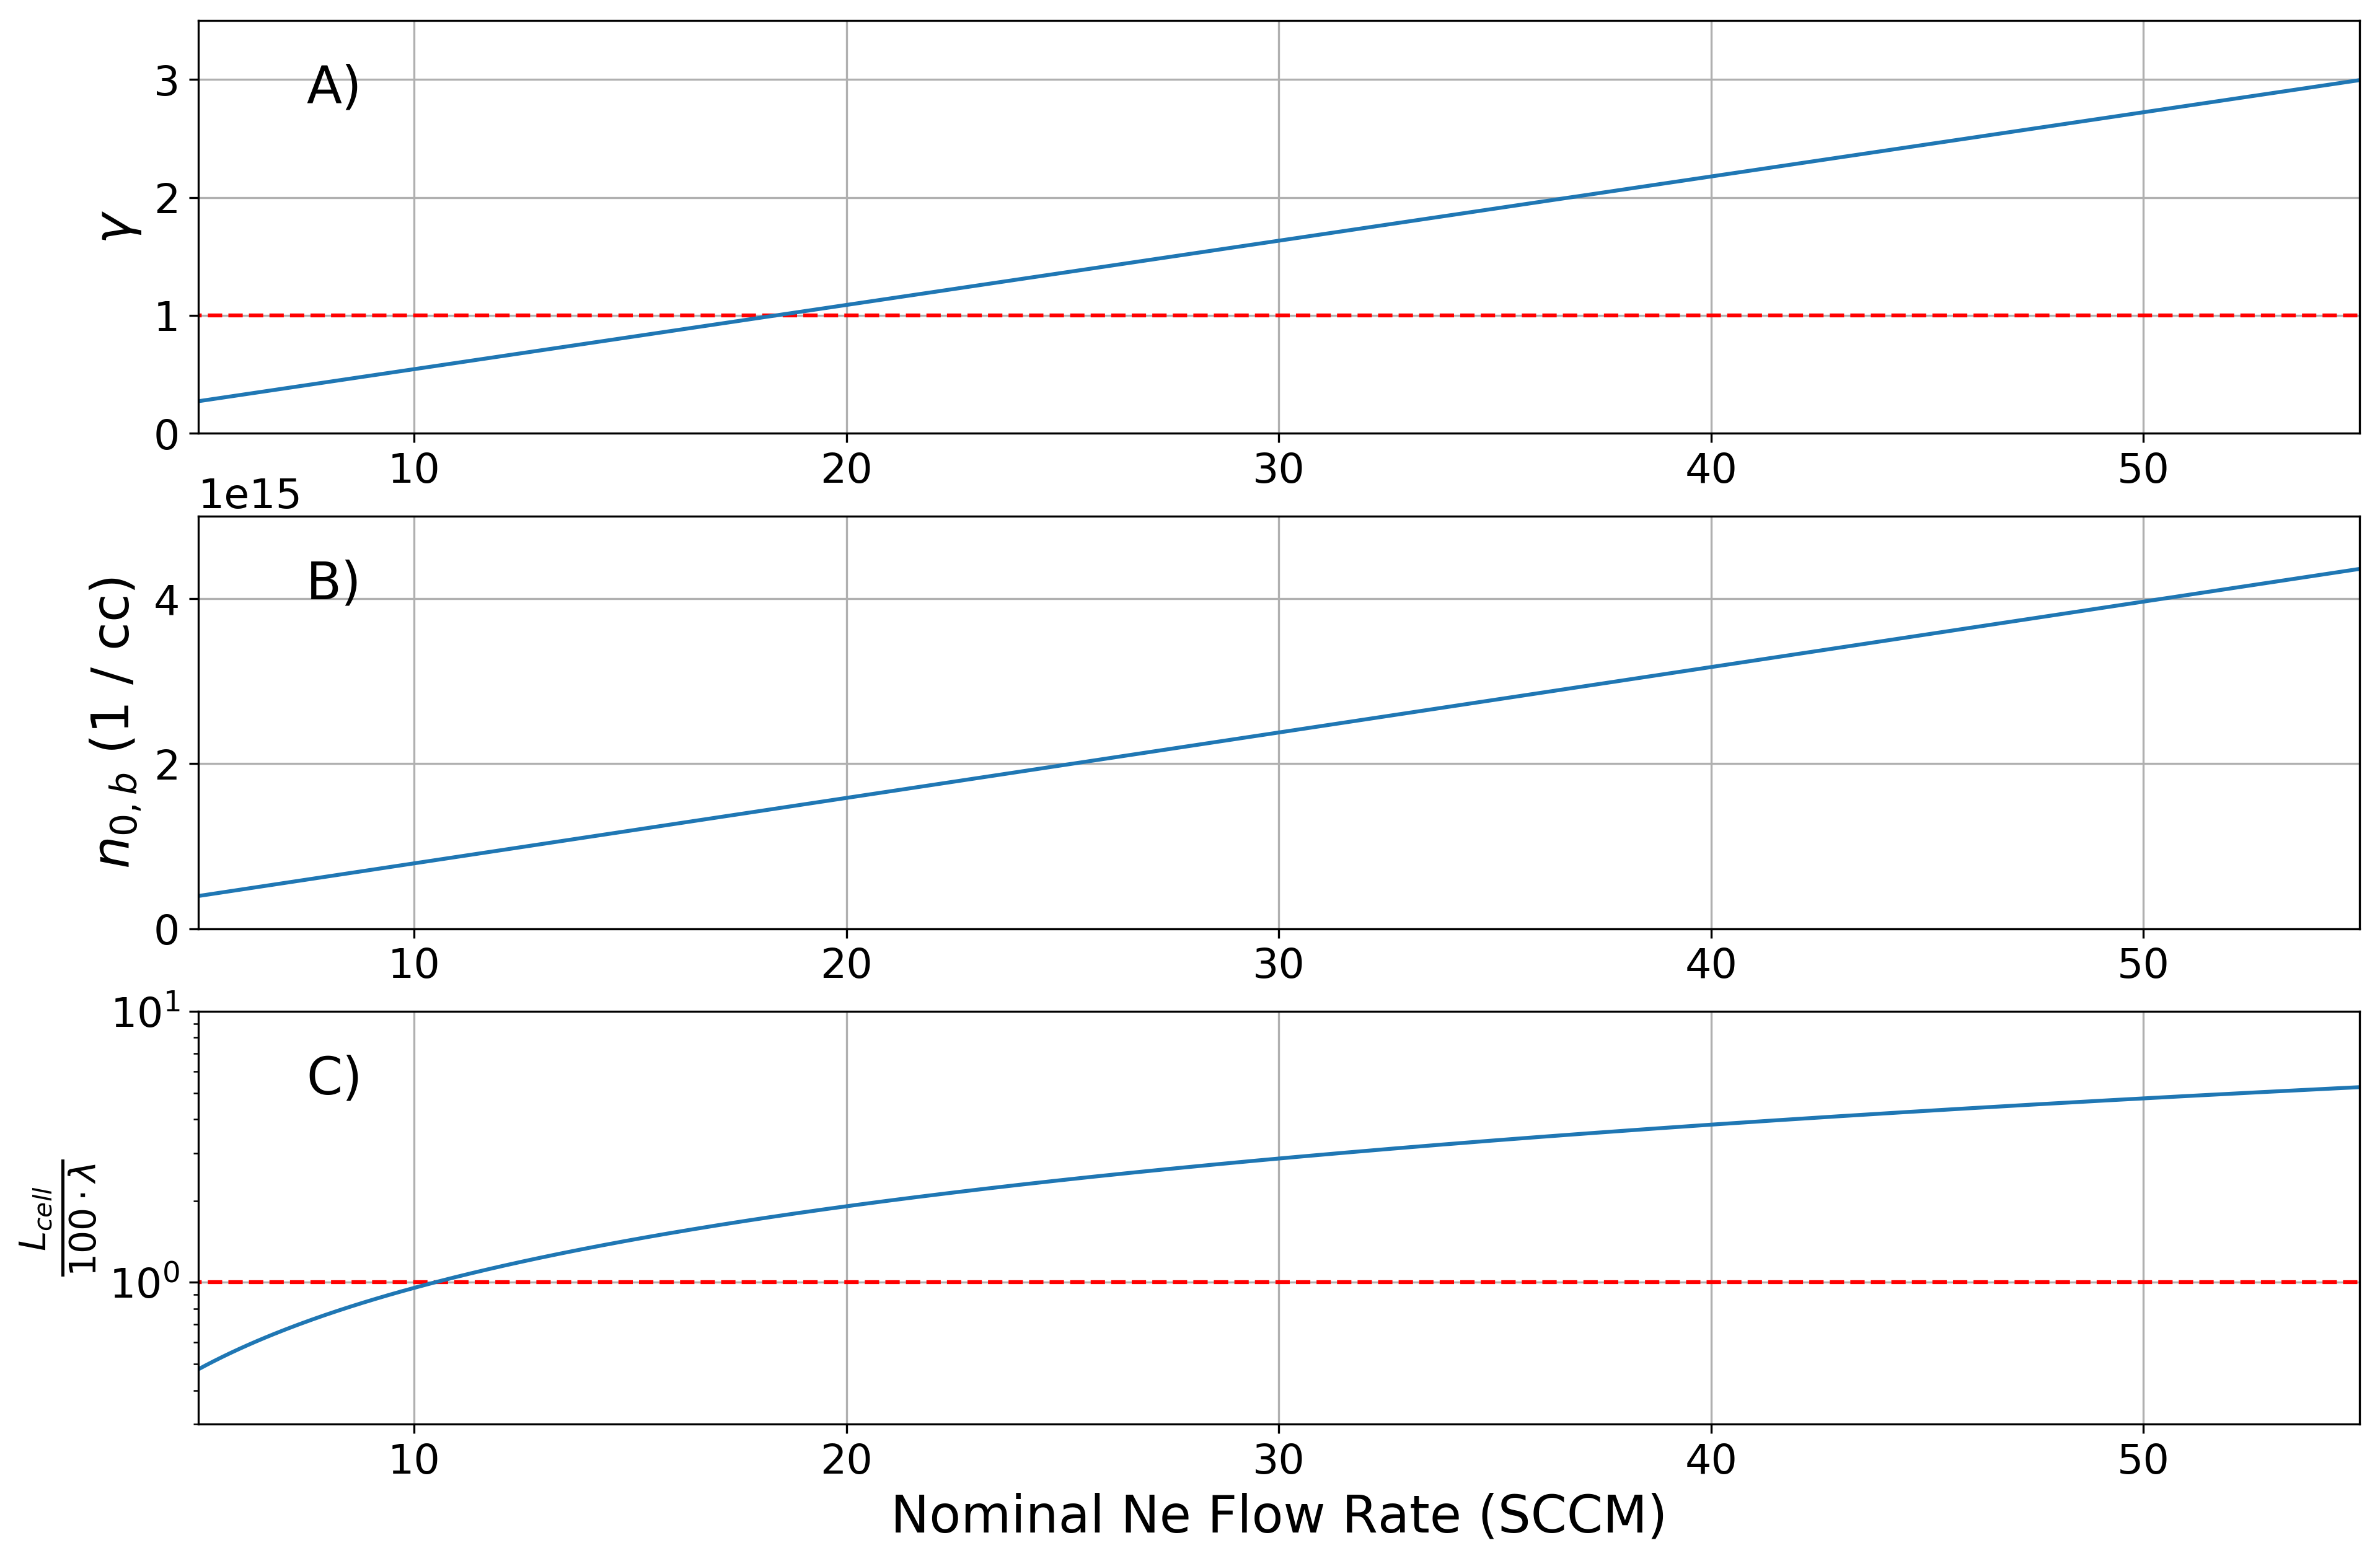
\includegraphics[width=1\textwidth]{images/CBGB_flow_characteristics.png}
	\caption{Theoretically derived buffer gas beam properties of interest given the physical dimensions of our cell in particular: $d_{\mathrm{aperture}} = 9$ mm. A) $\gamma$ extraction ratio, dotted red line indicates $\gamma = 1$ where hydrodynamic entrainment begins. B) Number density of buffer gas species within the experimental cell, given an enclosed back wall. The density of target species introduced should stay under 1\% of the buffer gas density for other properties to hold. C) Number of collisions a target species particle would expect before extraction out of the cell, the dotted red line indicates 100 collisions before extraction, when rotational degrees of freedom are characteristically thermalized.}
	\label{fig: buffer_gas_flow}
\end{figure}